\chapter{Introduction and Background}
\label{chap:introduction}

Spectrum sharing is a critical approach in modern wireless communications that allows multiple users, systems, or services to access the same frequency bands dynamically or concurrently while minimizing interference. Traditionally, spectrum allocation followed a static model where regulatory bodies, such as the  \gls{itu} or \gls{fcc}, assigned exclusive frequency bands to specific services, such as cellular networks, broadcasting, and military communications. However, with the exponential growth of wireless technologies—such as 5G, 6G, IoT, and satellite-based internet—this rigid allocation model has led to spectrum underutilization in some bands and congestion in others. Spectrum sharing mitigates this inefficiency by enabling more flexible and intelligent use of the available spectrum. 

There are various models of spectrum sharing, including \gls{dsa}, unlicensed spectrum sharing and \gls{lsa}. \gls{lsa} allows secondary users to access licensed spectrum under strict regulatory agreements, while \gls{dsa} employs cognitive radio technology to detect and utilize underutilized spectrum opportunistically. In unlicensed sharing, multiple users operate in shared bands  with interference management protocols. Techniques such as spectrum sensing, cooperative communication, and machine learning-based allocation further enhance the effectiveness of spectrum sharing by allowing real-time adaptation to spectrum availability. 

The need for spectrum sharing is driven by increasing spectrum scarcity, growing wireless traffic, and the demand for more efficient spectrum utilization. It enables cohabitation between different services, such as military and commercial applications, or between terrestrial and satellite networks, improving overall network capacity and reliability. Additionally, spectrum sharing reduces the need for costly spectrum auctions and facilitates innovation by allowing emerging technologies to access frequency bands that would otherwise remain unused. As wireless ecosystems evolve, spectrum sharing will play a pivotal role in ensuring sustainable and scalable connectivity while balancing regulatory, technical, and economic considerations.

Generative AI models have revolutionized machine learning by enabling the synthesis of high-quality data across various domains, including audio, image and text generation and speech synthesis. Unlike traditional discriminative models that learn decision boundaries, generative models aim to approximate complex data distributions, allowing them to generate realistic samples from learned representations. \gls{cnn}s have been the backbone of deep learning for visual data processing, excelling in tasks such as image and object detection, classification segmentation. By leveraging hierarchical feature extraction through convolutional layers, \gls{cnn}s capture spatial patterns, making them highly effective for structured data like images.



\section{Citizens Broadband Radio Service (CBRS)}
\label{sec:sec-1-1}

\gls{cbrs} in the United States refers to the unlicensed 150MHz spectrum in the 3.5 GHz band. \gls{cbrs} allows dynamic and efficient allocation of spectrum resources, fostering both commercial and public interest applications. \gls{cbrs} operates under a three-tiered hierarchy designed to prioritize and protect high-priority users while ensuring equitable access for lower-priority users:
 Incumbent, \gls{pal}, and \gls{gaa}. 

\begin{figure}[ht]
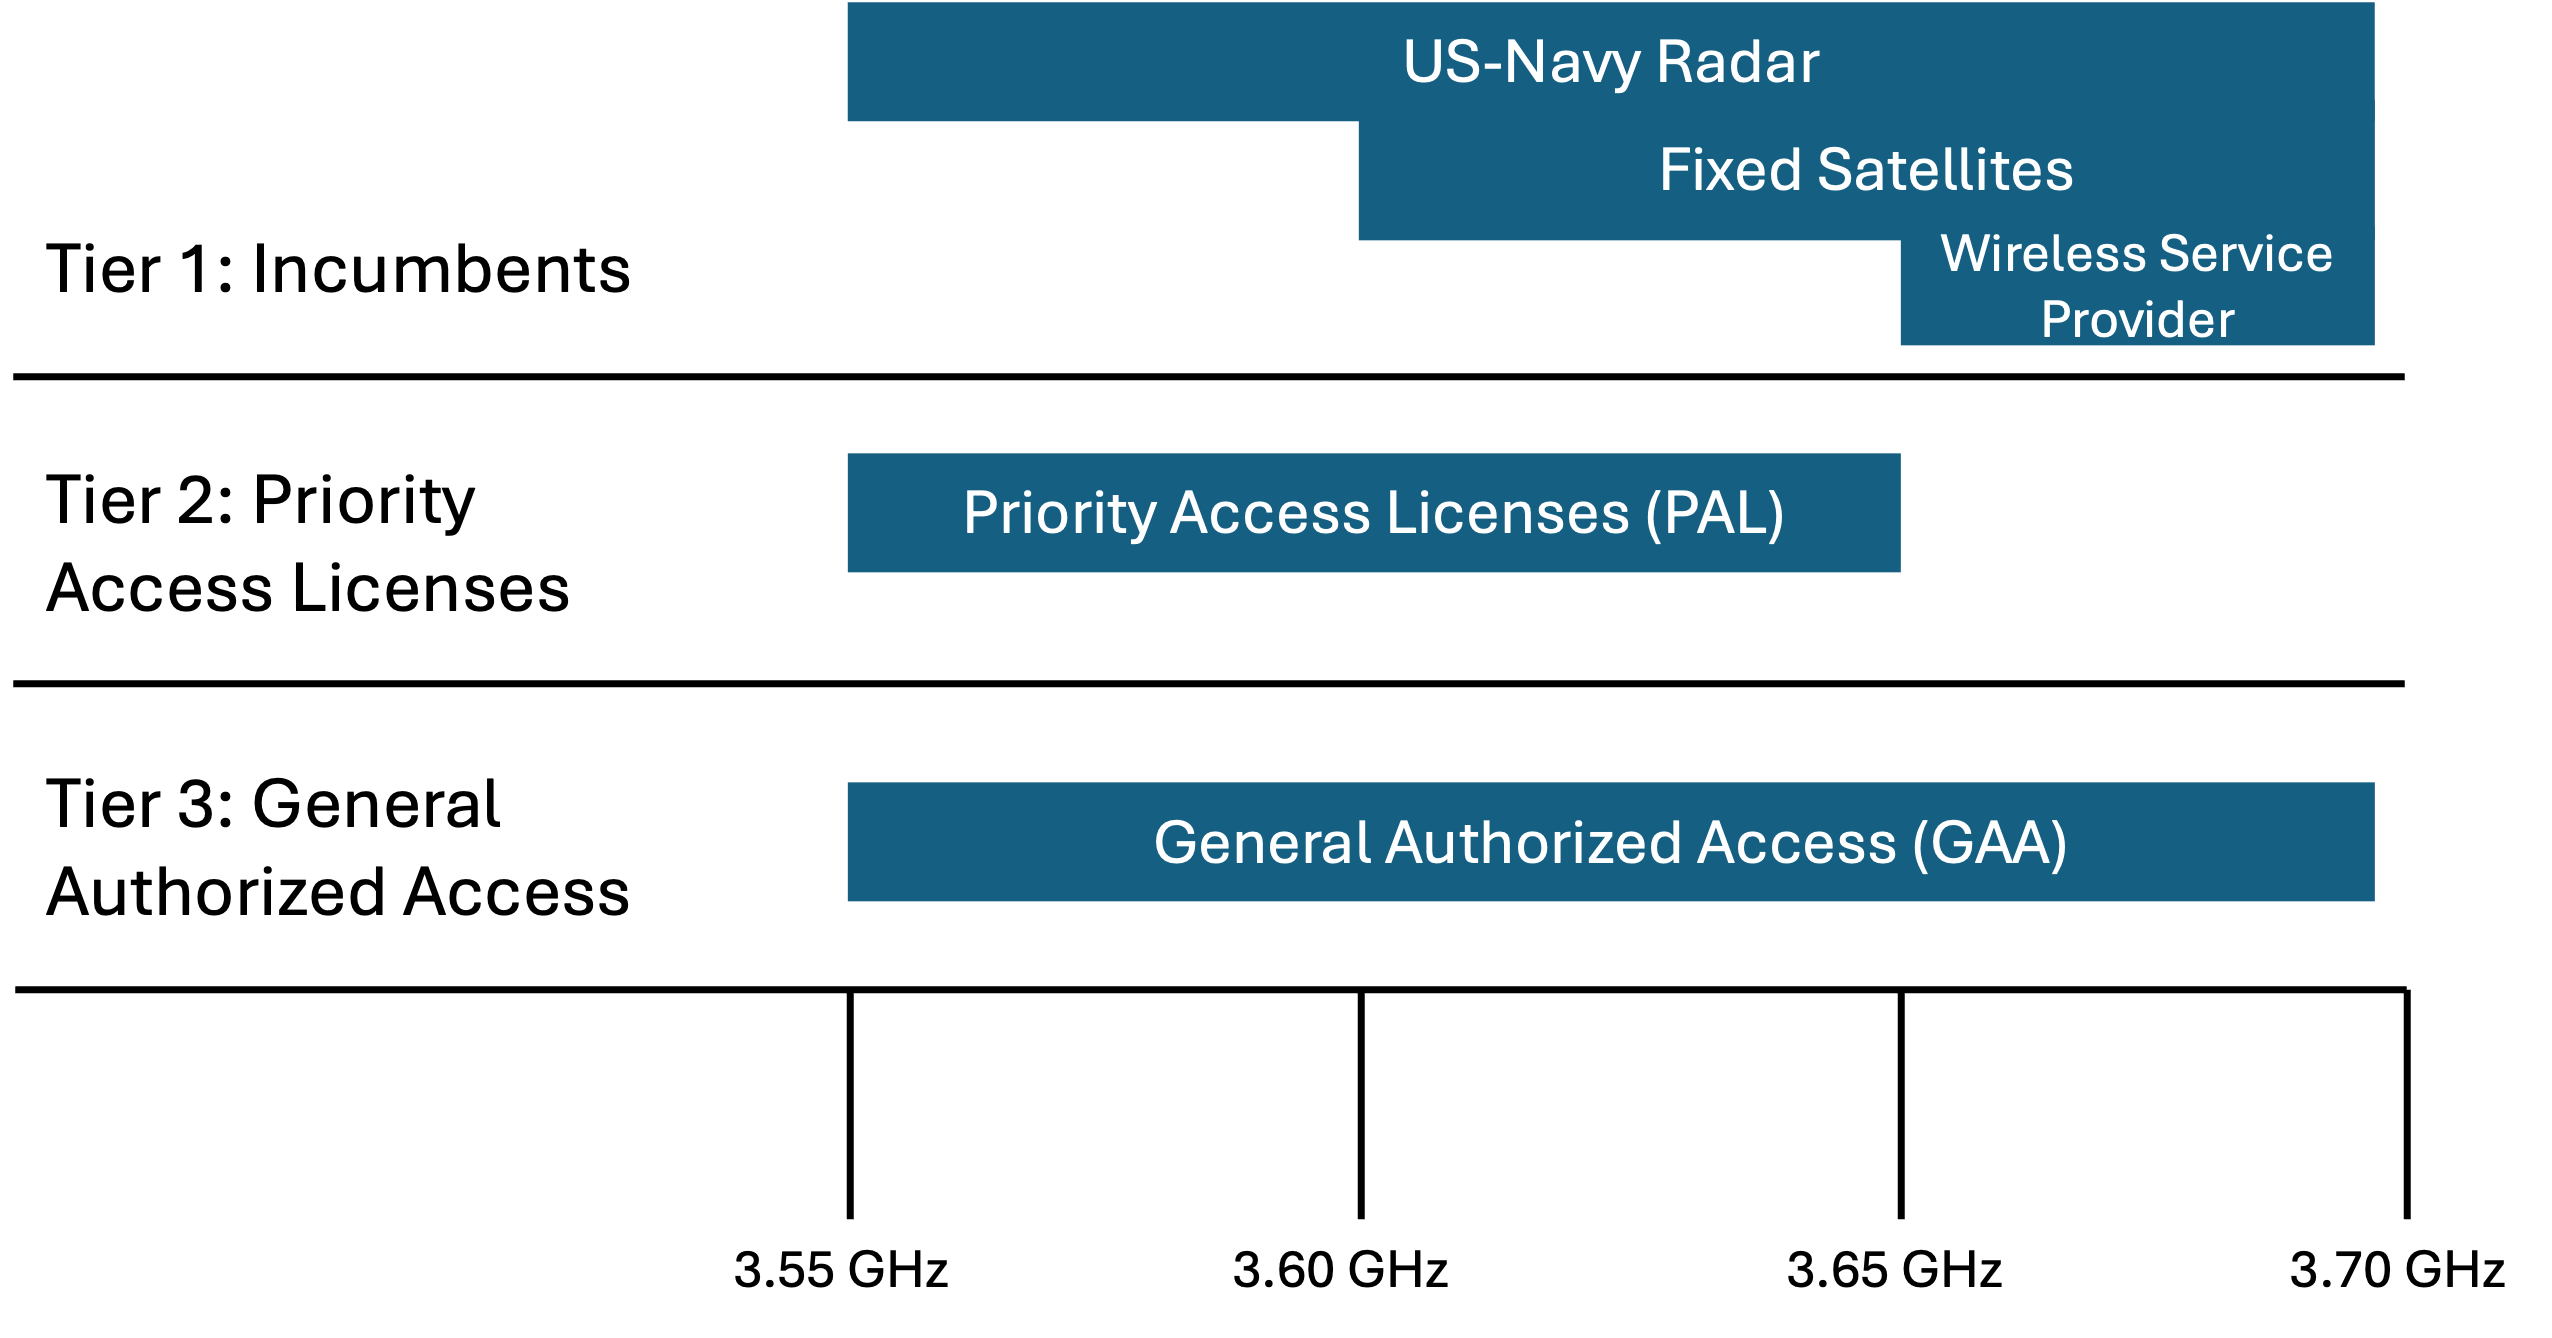
\includegraphics[width=\textwidth]{figures/cbrs_1.png}
\centering
\caption{The \gls{cbrs} spectrum }
\label{fig:cbrs-spectrum}
\centering
\end{figure}


Incumbent users include federal military radar systems and fixed satellite stations. These users have the highest priority and are granted uninterrupted access to the spectrum. Typically, these systems operate along coastal regions and require significant protection from interference.

\gls{pal} Users are licensed commercial users who acquire spectrum rights through an auction process. \gls{pal} licenses are granted for up to 10 MHz in a given geographic area and provide a level of protection from interference by lower-tier users. Common applications include private LTE/5G networks for enterprises, utilities, and healthcare.

\gls{gaa} users are the unlicensed users who can access the spectrum opportunistically in areas where it is not in use by Incumbent or \gls{pal} users.
\gls{gaa} users operate under strict rules to prevent interference with the higher-priority tiers. Figure 1.1 illustrates the three tiers of the \gls{cbrs} spectrum.

Since these tiers simultaneously use the \gls{cbrs} spectrum, the \gls{fcc} of the USA mandates that \gls{gaa} users must not cause interference with \gls{pal} or incumbent users, and \gls{pal} users must not cause interference with incumbent users. A \gls{sas} is used to manage the spectrum and avoid potential interference \cite{3}.

\gls{sas} is a cloud-based, automated frequency management system mandated by the \gls{fcc} to enforce \gls{cbrs} rules and ensure efficient use of the spectrum. \gls{sas} acts as a dynamic coordinator, regulating how the spectrum is shared and preventing interference between users across the three tiers.

The \gls{sas} continuously monitors the spectrum usage and allocates channels dynamically to users based on their tier. Incumbent users are always given precedence, followed by \gls{pal} users, and then \gls{gaa} users.
To prevent collision scenarios, particularly involving Incumbent users, \gls{sas} currently employs several mechanisms, including continuous monitoring, spectrum reallocation for non-priority users, and preemption for Incumbent users.

Preventing interference is crucial in \gls{cbrs} operations. \gls{sas} enforces a priority hierarchy, ensuring \gls{gaa} users access spectrum only when \gls{pal} and Incumbent users are inactive. If a higher-priority user requires access, \gls{sas} reallocates \gls{gaa} users dynamically. \gls{pal} users are similarly protected through exclusive spectrum assignments \cite{4}.  

\section{Background}

\gls{gan}s and diffusion-based generative models have gained significant traction for various applications, including spectrogram augmentation and audio synthesis. In \cite{14}, \gls{gan}-based models were employed for Radar spectrogram augmentation, leveraging a \gls{jdl} module for injecting diversity into synthetic data. While effective for enhancing dataset variability, the reliance on adversarial training often poses challenges in terms of stability and convergence, particularly in complex spectrogram domains.


The work in \cite{9} conducted a multimodal comparison of latent Diffusion Models (\gls{ddpm}s) and \gls{gan}s for medical image synthesis. Their results demonstrated the superiority of latent \gls{ddpm}s over Least Squares \gls{gan} and Variational Autoencoder \gls{gan}, particularly in generating high-quality, diverse images. While this comparison offers insights into the potential of diffusion models, its application was limited to medical imaging and did not address the challenges of dynamic spectrum scenarios, such as those found in \gls{cbrs}.

The U-Net architecture, proposed in Imagen \cite{16} and later adapted in \cite{17}, has shown promise for spectrogram-based high-quality audio synthesis. These approaches exploit the hierarchical encoding-decoding structure of U-Nets to generate fine-grained audio spectrograms but have not been extended to the domain of spectrum-sharing systems or collision detection in \gls{cbrs}.

Effective \gls{cbrs} management relies on robust collision detection, yet traditional rule-based methods struggle in dynamic environments due to scalability and adaptability challenges. Deep learning-based classification offers a promising alternative, but the scarcity of collision data limits training \cite{5}.  

To address this, we propose a novel spectrum-sharing system that generates spectrogram images of collision scenarios using \gls{gan} \cite{6}, \gls{ddpm} \cite{7}, and \gls{vq-vae} \cite{8}. These images will train a \gls{cnn} to detect collisions and alert \gls{sas}. 

We evaluate the generative models by comparing their impact on \gls{cnn} classification accuracy and data diversity. Then we simulate a \gls {cbrs} environment using MATLAB which uses \gls{drl} for instead of a \gls{sas} to assign channels to users in a rapidly changing environment. While \gls{gan}s and VAEs have been used to address data limitations, diffusion models have shown state-of-the-art results in natural image generation \cite{9}. However, a direct use generative AIs with \gls{cnn} for interference detection and \gls{drl} for channel allocation is unexplored.  

This work employs conditional \gls{gan}, conditional \gls{ddpm}, and \gls{vq-vae} models to generate visualized \gls{cbrs} datasets and compares their performance based on \gls{cnn} classification accuracy.  

The key contributions of this study are:
\begin{enumerate}
    \item Introduce a scalable and generalizable spectrum-sharing system for a dynamic \gls{cbrs} environment.
    \item Use Generative models to generate visualized waveforms of a \gls{cbrs} system.
    \item Make a quantitative comparison of three of the most popular generative models currently available, in generating frequency spectrogram images.
    \item Use \gls{drl} based channel allocation system with a \gls{cnn} based collision detection system to manage the \gls{cbrs} environment.
\end{enumerate}


This document consists of the following: Chapter 2 has the background explanations and the system architecture of this thesis and the Chapter 3 anaylze the results, performance of the genarative models and the \gls{drl} agent. Chapter 4 includes a discussion of the results and Chapter 5 includes the conclusion and future work.

